\chapter[Software processes]{\thechapter. Software processes}
\section{Overview}
Software process is defined as complex and rich set of sequence activities, that embody certain strategies to develop and maintain of software. Although each process embodies different strategies, there are common fundamental activities:
\begin{itemize}
\item Software specification - the functional and non functional specifications and constraints on its operations.
\item Software development - software development within the scope software specifications.
\item Software validation - the software product validated to software specification.
\item Software evolution - all updates required to meet changing customer needs.
\end{itemize}
Every process is evolved with the exploiting the capability of making the right judgements and presenting with enough creativity by the development team, thus different processes solutions could be taken and applied within one project. To improve the strategies of a certain process it is necessary to evaluate the success of the project, to try avoiding and repeating those wrong decisions in the future, which leads to standardization of the process and creating of a process model.\\ 
Based on the angle of attention, the set of process model could be subdivided into three main groups of: product, process and development.
\newpage
\section{Software product model} 
Also know as life cycle models, describing each step done during the software development activities often as stages and are independent of software application domain, programming language and context. 
\subsection{Waterfall}
Is a phase model, resembling finite state machine, with downward sequence of transition through the common fundamental  activities as shown in Figure 1.1. Each stage results as a deliverable, which servers as the initial inputs for the following stage. It is not possible to continue with the development and move to the next stage, if the previous one is not successfully completed.
\begin{center}
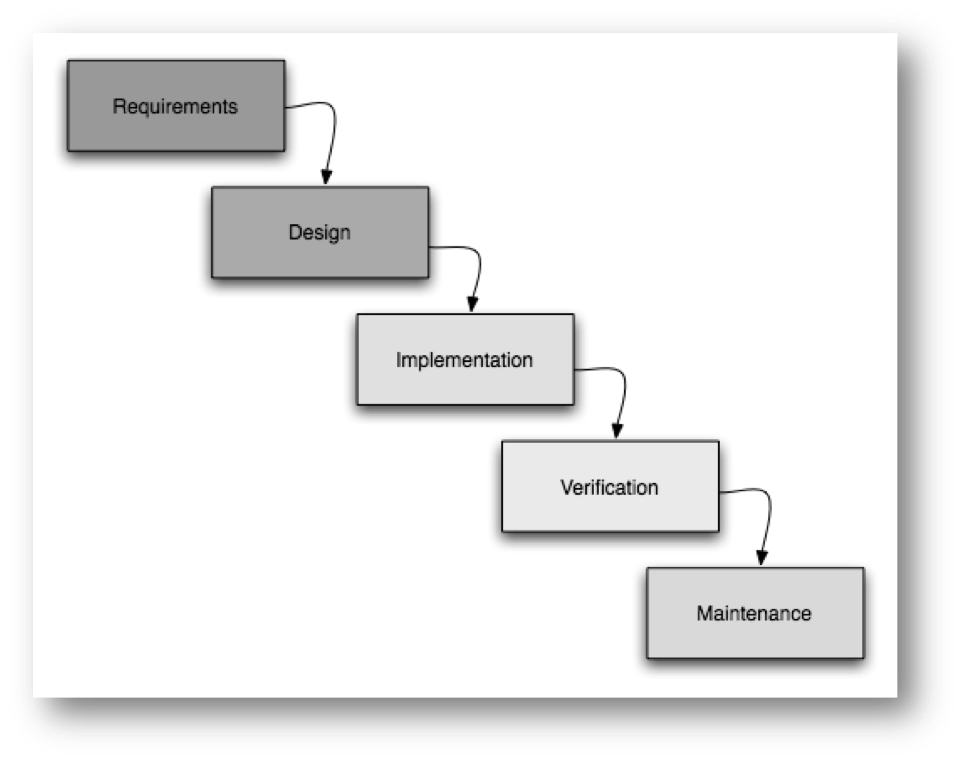
\includegraphics[scale=0.75]{Images/Waterfall_model.png}\\
Figure 1.1\footnote{Quelle: Wikipedia} - Waterfall model
\end{center}
{\bf Requirements -} Consulting with the user, the system specification and constrain are defined in detailed.\\
{\bf Design -} An overall system architecture is established and the software design describes the fundamental software abstraction.\\
{\bf Implementation -} The software design results as a set of programs.\\
{\bf Verification -} The set of program is test as a while system to insure the software requirements.\\
{\bf Maintenance -} Every maintenance process that could possible occur.\\ \\
The well documented stages is the advantage of the waterfall model. As disadvantage could be seen the inability of flexible partitioning of the project into distinct stages, which makes it difficult to respond to changing customer requirements. That why this model shall be only used in case of well understood requirement and for helping to structure and manage the development of large systems in complex organizations.\\
\subsection{V-Model}
The V-Model could be seen as an extension of the waterfall model described in the previous section of this chapter. The sequence of transitions between the phases is done at first at the left side of the stream, which acts as a input document for the right side of the stream as shown in Figure 1.2.\\ \\
Every design element is traceable from defined to tested system requirements. Thus every phase done shall cover a requirement, leaving no room for unnecessarily done stages and everything that is necessary is being accomplished. 
\begin{center}
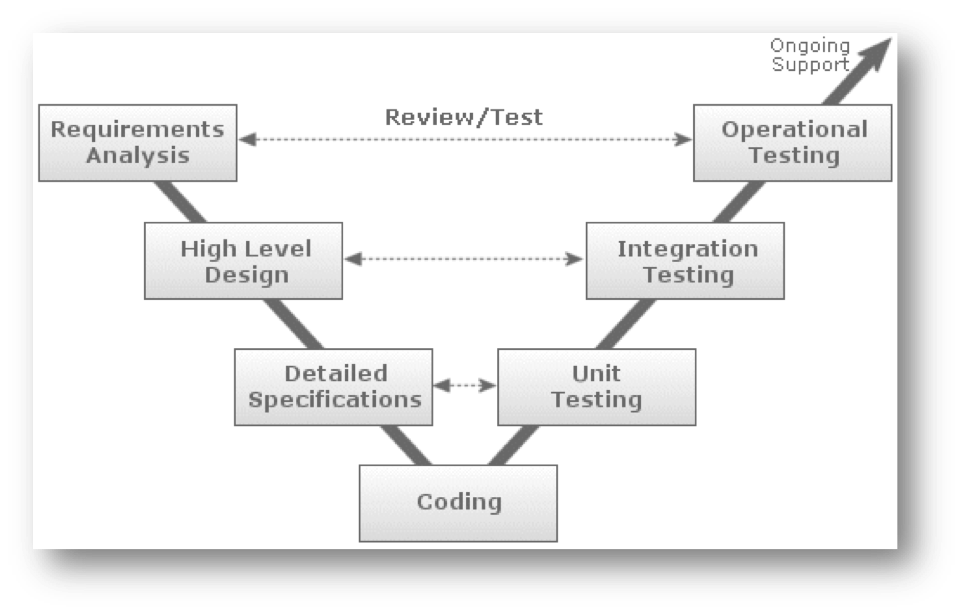
\includegraphics[scale=0.75]{Images/V_Model_model.png}\\
Figure 1.2\footnote{Quelle: http://sumeetanand.net/} - V-Model
\end{center}
The left side of the stream represents the  definition of system specification. The right side represents the validation stream where the systems are being tested. The bottom stream represents the development stream.\\ \\
This model does not covers the maintenance and disposal of the system, only the planing and preparation.
\section{Software development model} 
These software development models represent an evolutionary revision to the software product models\footnote{MacCormack 2001} due to the availability of new software development strategies such as: reusable software, application generations, software prototyping.\\
\subsection{Software prototyping}
It is a technique for providing a reduced functionality or limited performance version of a software system early in its development\footnote{Balzer 1983, Budde 1984, Hekmatpour 1987}.As a fundamental point for development of prototypes is the use of a software functional specification, that is later simulate, analyzed and evaluated.\\ \\
Software prototypes come in different forms, including and represent an incomplete version of the software being develop.\\
{\bf Mockups -} they look like the end product with not functionality.\\
{\bf Throwaway -} creating a model that could provide with a quick user feedback regarding the requirements.\\
{\bf Evolutionary  -} robust and functional part of the system. This prototypes  are being continually refine and rebuilt.\\
{\bf Incremental  -} each requirement is build as a separated prototype. At the end all the parts are combine to build up the end product.\\
\\
Taking advantage of prototypes in the software development could reduce time, cost, improve and increase user involvement, provide at an early stage with valuable user feedback and specification, improve the quality of requirements and specifications provided to the developers.\\ \\
The main disadvantage and back draw is that the user could get confused between the real product and the prototype.\\
\subsection{Joint application development}
Joint application development (JAD) represents a technique for engaging a group or team of software developers, testers, customers and prospective end users in a collaborative workshop. Following a strict agenda in order to guarantee that any difficulties or difference between the users and developers will be sorted-out.\\ \\
The workshop is based on four ideas:\\
{\bf Requirements review -} the people involve with the development of the system, have the best understanding of that job.\\
{\bf Development review -} the developers have the best inside of the capability and possibility of the technology.\\
{\bf Evolutionary review  -} the actual user of common system haven a valuable insight on the role of a system in the community.\\
{\bf Collaborative review -} when all those groups work together on the project as equal partners.\\
\\
The advantage of JAD can result in more accurate system specification and better understanding system requirements. A drawback is it more expensive and time consuming process, in which there a lot of scope for inter-personal conflicts.
\newpage
\section{Software process model}
Set of software process model includes models that are acting like scripts, programs or automated processes.
\subsection{Iterative and incremental model}
This model based is on the idea of Divide and Conquer and it is an extension of the Waterfall model. The first phase is to divide the system in small pieces and schedule them to be developed over time, that is done during the incremental stage. The next phase is the iterative one, in which the time is taking in order to improve, refine and to adjust them to the changing software requirements.
\begin{center}
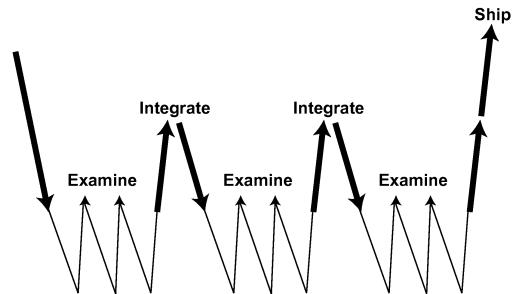
\includegraphics[scale=0.75]{Images/Iterative_development_model.png}\\
Figure 1.3\footnote{Quelle: CrossTalk} - Iterative and incremental model
\end{center}
\subsection{Spiral model}
The spiral model of software development and evolution represents a risks-driven approach to software process analysis and structuring\footnote{Boehm 1987, Boehm et al,1998}.\\ \\The spiral is a iterative development cycles, with inner cycles of spiral representing early system analysis and prototyping, the outer cycles representing the software life cycle as shown in Figure 1.3\footnote{Quelle: Massachusetts institute of technology}.\\
\begin{center}
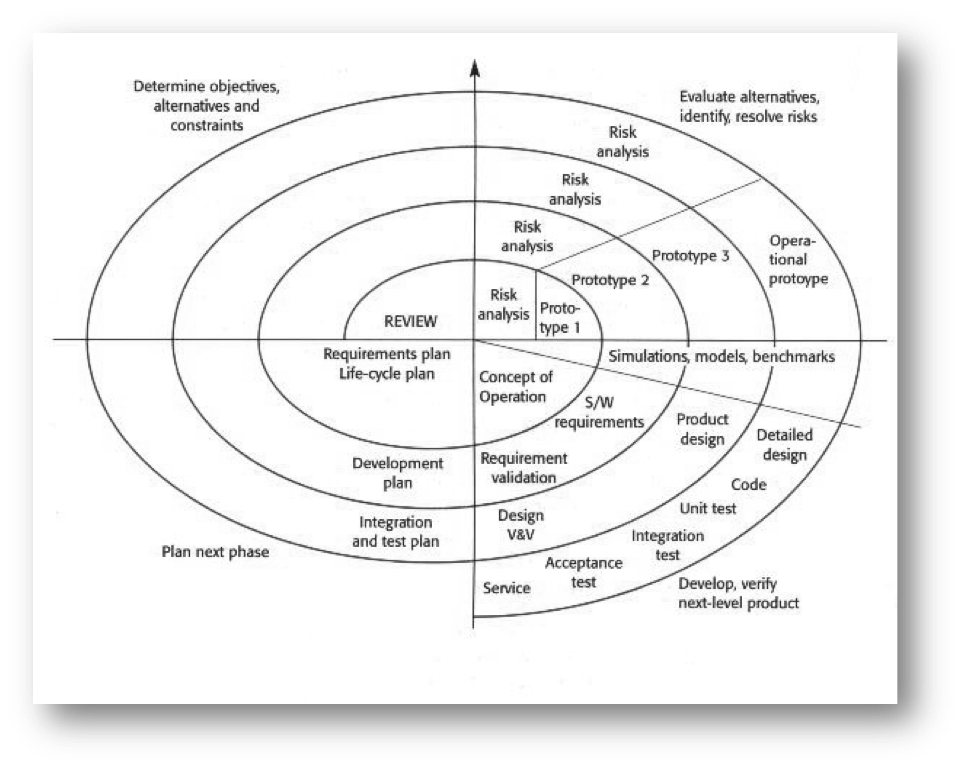
\includegraphics[scale=0.75]{Images/Spiral_model.png}\\
Figure 1.3 - Spiral model
\end{center}
{\bf Objective settings -} specific settings and risks are defined, a management plan is drawn up.\\
{\bf Risk analysis -} detailed analysis and evaluation for each of the defined risk in the previous loop, possibility of risk assessment.\\
{\bf Development and validation -} a development model is chosen, usually the waterfall model.\\
{\bf Planing -}  the review the status of project, if is decided to continue, a plan are created for the next phase.\\
\\
The advantage of a risk driven approach is that it avoids many of common difficulties.Using the The primary advantage is that its risk driven approach. The main drawback is the risk assessment and evaluation, if it is done incorrectly, it could lead to fatal end for the project.
















